\documentclass[12pt,a4paper]{article}
\usepackage[utf8]{vietnam}
\usepackage{amsmath,amssymb}
\usepackage{tabularx}
\usepackage{graphicx}
\usepackage{tikz}
\usetikzlibrary{calc,arrows.meta}
\usepackage{xcolor}
\usepackage{enumitem}
\usepackage{fancyhdr}
\usepackage[top=0.8cm, bottom=0.8cm, left=1.2cm, right=1.2cm]{geometry}
\usepackage[dethi]{ex_test}
\SAOPTN{widthSA=2.6,heightSA=0.62}

\setlength{\headheight}{15pt}
\setlength{\parskip}{0pt}

\pagestyle{fancy}
\fancyhf{}
\rhead{\textit{Môn Toán 7 -- Đề số 13}}
\lhead{\textit{Bộ đề ôn tập Giữa học kì I}}
\cfoot{\thepage}

\begin{document}

% --- KHUNG TIÊU ĐỀ ĐỀ THI ---
\noindent
\begin{tabularx}{\linewidth}{X r}
\textbf{TRƯỜNG THCS: \dotfill} & \textbf{ĐỀ KIỂM TRA ĐỊNH KỲ GIỮA HỌC KỲ I} \\
\textbf{Họ và tên: \dotfill} & \textbf{NĂM HỌC 2026 -- 2027} \\
\textbf{Lớp: \dotfill \quad SBD: \dotfill} & \textbf{Môn: TOÁN 7} \\
& \textit{Thời gian làm bài: 90 phút (không kể thời gian phát đề)}
\end{tabularx}

\vspace{1mm}
\noindent
\begin{tabularx}{\linewidth}{|p{3.5cm}|X|}
\hline
\centering\textbf{Điểm số} & \centering\textbf{Lời nhận xét của thầy cô giáo} \tabularnewline
\rule{0pt}{0.8cm} & \\
\hline
\end{tabularx}

\vspace{1.5mm}
\begin{center}
\textbf{\large ĐỀ SỐ 13}
\end{center}

\noindent\textbf{\large PHẦN I. CÂU TRẮC NGHIỆM NHIỀU PHƯƠNG ÁN LỰA CHỌN (3,0 điểm)}

\textit{Thí sinh trả lời từ câu 1 đến câu 12. Mỗi câu hỏi chỉ chọn một phương án đúng nhất và ghi vào bảng đáp án.}

\vspace{1mm}
\begin{ex}
Kết quả của biểu thức $-\dfrac{3}{4} - \left(-\dfrac{1}{4}\right) - \dfrac{8}{7} - \dfrac{4}{7} - \dfrac{7}{7} + \dfrac{1}{3}$... sau khi thu gọn các phân số cùng mẫu là:
\choice
{$-\dfrac{37}{7}$}
{\True $-3$}
{$-\dfrac{25}{28}$}
{$-4$}
\end{ex}

\begin{ex}
Kết quả của phép tính $\left(-\dfrac{2}{3}\right)^3$ là:
\choice
{$-\dfrac{6}{9}$}
{$\dfrac{8}{27}$}
{\True $-\dfrac{8}{27}$}
{$\dfrac{6}{9}$}
\end{ex}

\begin{ex}
Một hồ bơi có dạng hình hộp chữ nhật có các kích thước lần lượt là $15\text{ m}; 10\text{ m}; 1{,}8\text{ m}$. Thể tích hồ bơi là:
\choice
{\True $270\text{ m}^3$}
{$180\text{ m}^3$}
{$240\text{ m}^3$}
{$90\text{ m}^3$}
\end{ex}

\begin{ex}
Cho biểu thức $-\left(\dfrac{1}{12} - \dfrac{2}{5}\right)$, khi bỏ dấu ngoặc ta được:
\choice
{$\dfrac{1}{12} - \dfrac{2}{5}$}
{$-\dfrac{1}{12} - \dfrac{2}{5}$}
{$\dfrac{1}{12} + \dfrac{2}{5}$}
{\True $-\dfrac{1}{12} + \dfrac{2}{5}$}
\end{ex}

\begin{ex}
\immini{
Quan sát trục số sau, điểm $A$ biểu diễn số hữu tỉ nào?
\choice
{$1{,}3$}
{$4$}
{\True $\dfrac{4}{3}$}
{$\dfrac{4}{5}$}
}{
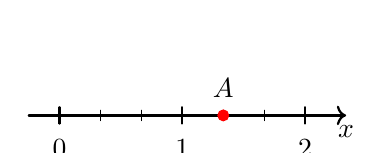
\begin{tikzpicture}[scale=1.3, line cap=round, line join=round]
    \draw[thick, ->] (-0.3,0) -- (2.8,0) node[below] {$x$};
    \foreach \x/\label in {0/0, 1.2/1, 2.4/2} {
        \draw[thick] (\x, 0.08) -- (\x, -0.08) node[below=2pt] {$\label$};
    }
    \foreach \x in {0.4, 0.8, 1.6, 2.0} {
        \draw (\x, 0.05) -- (\x, -0.05);
    }
    \filldraw[red] (1.6, 0) circle (1.5pt) node[above=3pt, black] {$A$};
\end{tikzpicture}
}
\end{ex}

\begin{ex}
\immini{
Cho hình vẽ dưới đây, góc đối đỉnh với $\widehat{xOy}$ là góc nào?
\choice
{\True $\widehat{x'Oy'}$}
{$\widehat{xOy'}$}
{$\widehat{x'Oy}$}
{$\widehat{xOy}$}
}{
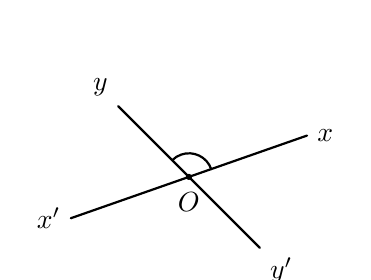
\begin{tikzpicture}[scale=0.75, line cap=round, line join=round]
    \coordinate (O) at (0,0);
    \draw[thick] (-2, -0.7) node[left] {$x'$} -- (2, 0.7) node[right] {$x$};
    \draw[thick] (-1.2, 1.2) node[above left] {$y$} -- (1.2, -1.2) node[below right] {$y'$};
    \filldraw[black] (O) circle (1.2pt) node[below=2pt] {$O$};
    \draw[thick] (O) ++(19.3:0.4) arc (19.3:135:0.4);
\end{tikzpicture}
}
\end{ex}

\begin{ex}
Qua một điểm $M$ nằm ngoài đường thẳng $a$, kẻ được bao nhiêu đường thẳng song song với đường thẳng $a$?
\choice
{Có vô số đường thẳng}
{Không có đường thẳng nào}
{Có hai đường thẳng}
{\True Chỉ có một đường thẳng}
\end{ex}

\begin{ex}
Cho $\triangle ABC = \triangle DEF$. Biết $\widehat{A} = 33^\circ$. Khi đó:
\choice
{\True $\widehat{D} = 33^\circ$}
{$\widehat{B} = 33^\circ$}
{$\widehat{E} = 33^\circ$}
{$\widehat{F} = 33^\circ$}
\end{ex}

\newpage
\begin{ex}
Giá trị của $|-3|$ bằng:
\choice
{$-3$}
{\True $3$}
{$\dfrac{1}{3}$}
{$-\dfrac{1}{3}$}
\end{ex}

\begin{ex}
Làm tròn số $1{,}3781$ với độ chính xác $0{,}005$ được kết quả là:
\choice
{$1{,}37$}
{$1{,}4$}
{$1$}
{\True $1{,}38$}
\end{ex}

\begin{ex}
Số đỉnh của hình hộp chữ nhật là:
\choice
{$6$}
{\True $8$}
{$10$}
{$12$}
\end{ex}

\begin{ex}
\immini{
Cho hình vẽ sau, biết $a \parallel b$ và $\widehat{A} = 45^\circ$. Số đo của góc $\widehat{B}_1$ bằng bao nhiêu?
\choice
{$145^\circ$}
{$45^\circ$}
{$35^\circ$}
{\True $135^\circ$}
}{
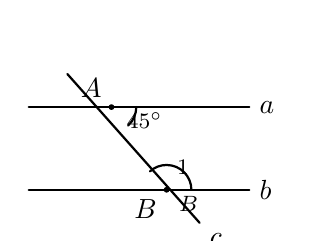
\begin{tikzpicture}[scale=0.7, line cap=round, line join=round]
    \draw[thick] (-1.5, 1.5) -- (2.5, 1.5) node[right] {$a$};
    \draw[thick] (-1.5, 0) -- (2.5, 0) node[right] {$b$};
    \draw[thick] (-0.8, 2.1) -- (1.6, -0.6) node[below right] {$c$};
    \filldraw[black] (0, 1.5) circle (1.2pt) node[above left] {$A$};
    \filldraw[black] (1.0, 0) circle (1.2pt) node[below left] {$B$};
    % Angle A
    \draw[thick] (0, 1.5) ++(0:0.45) arc (0:-48:0.45);
    \node[font=\footnotesize] at (0.6, 1.25) {$45^\circ$};
    % Angle B1
    \draw[thick] (1.0, 0) ++(0:0.45) arc (0:132:0.45);
    \node[font=\footnotesize] at (1.3, 0.4) {$1$};
    \node[font=\footnotesize] at (1.4, -0.25) {$B$};
\end{tikzpicture}
}
\end{ex}


\vspace{1mm}
\noindent\textbf{BẢNG TRẢ LỜI TRẮC NGHIỆM PHẦN I:}
\begin{center}
\begin{tabular}{|c|c|c|c|c|c|c|c|c|c|c|c|c|}
\hline
\textbf{Câu} & \textbf{1} & \textbf{2} & \textbf{3} & \textbf{4} & \textbf{5} & \textbf{6} & \textbf{7} & \textbf{8} & \textbf{9} & \textbf{10} & \textbf{11} & \textbf{12} \\
\hline
\textbf{Chọn} & \rule{0pt}{0.48cm} & & & & & & & & & & & \\
\hline
\end{tabular}
\end{center}
\vspace{1mm}

\setcounter{ex}{0}
\noindent\textbf{\large PHẦN II. CÂU TRẮC NGHIỆM ĐÚNG SAI (2,0 điểm)}

\textit{Thí sinh trả lời câu 1 và câu 2. Trong mỗi ý a), b), c), d) ở mỗi câu, thí sinh chọn đúng hoặc sai.}

\vspace{1mm}
\begin{ex}
Cho biểu thức $Q = \left(-\dfrac{1}{3}\right)^2 \cdot 9 + \left|-\dfrac{3}{5}\right| : \dfrac{3}{5} - \dfrac{1}{2}$. Xét tính đúng sai của các mệnh đề sau:
\choiceTF
{\True Giá trị của lũy thừa $\left(-\dfrac{1}{3}\right)^2$ bằng $\dfrac{1}{9}$}
{Giá trị tuyệt đối $\left|-\dfrac{3}{5}\right|$ bằng $-\dfrac{3}{5}$}
{\True Kết quả của phép tính $\dfrac{3}{5} : \dfrac{3}{5}$ bằng $1$}
{\True Giá trị của biểu thức $Q$ bằng $\dfrac{3}{2}$}
\end{ex}

\begin{ex}
\immini{
Quan sát hình vẽ, biết $MN \perp yy'$ tại $M$ và $MN \perp zz'$ tại $N$; đường thẳng $xx'$ cắt $yy'$ tại $A$ và cắt $zz'$ tại $B$ sao cho góc $\widehat{xAy'} = 60^\circ$. Xét tính đúng sai của các mệnh đề sau:
\choiceTF
{\True Hai đường thẳng $yy'$ và $zz'$ song song với nhau}
{\True Số đo của góc $\widehat{yAB}$ bằng $60^\circ$}
{Số đo của góc $\widehat{ABz'}$ bằng $120^\circ$}
{\True Hai góc $\widehat{y'AB}$ và $\widehat{ABz}$ là hai góc so le trong và đều có số đo bằng $120^\circ$}
}{
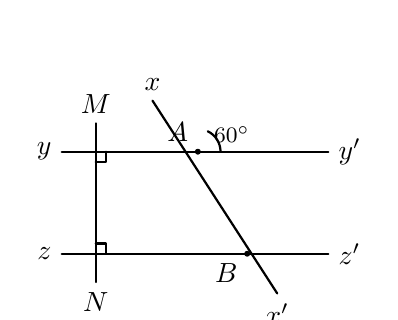
\begin{tikzpicture}[scale=0.72, line cap=round, line join=round]
    % Lines yy' and zz'
    \draw[thick] (-2.2, 1.8) node[left] {$y$} -- (2.5, 1.8) node[right] {$y'$};
    \draw[thick] (-2.2, 0) node[left] {$z$} -- (2.5, 0) node[right] {$z'$};
    % MN perpendicular
    \draw[thick] (-1.6, 2.3) node[above] {$M$} -- (-1.6, -0.5) node[below] {$N$};
    \draw[thick] (-1.6, 1.8) ++(0,-0.18) -- ++(0.18,0) -- ++(0,0.18);
    \draw[thick] (-1.6, 0) ++(0,0.18) -- ++(0.18,0) -- ++(0,-0.18);
    % Line xx'
    \draw[thick] (-0.6, 2.7) node[above] {$x$} -- (1.6, -0.7) node[below] {$x'$};
    \filldraw[black] (0.2, 1.8) circle (1.2pt) node[above left] {$A$};
    \filldraw[black] (1.07, 0) circle (1.2pt) node[below left] {$B$};
    % Angle xAy' = 60
    \draw[thick] (0.2, 1.8) ++(0:0.4) arc (0:64:0.4);
    \node[font=\footnotesize] at (0.8, 2.1) {$60^\circ$};
\end{tikzpicture}
}
\end{ex}


\noindent\textbf{BẢNG TRẢ LỜI PHẦN II:}
\begin{center}
\begin{tabular}{|c|c|c|c|c||c|c|c|c|c|}
\hline
\textbf{Câu 1} & \textbf{a)} & \textbf{b)} & \textbf{c)} & \textbf{d)} & \textbf{Câu 2} & \textbf{a)} & \textbf{b)} & \textbf{c)} & \textbf{d)} \\
\hline
\textbf{Đ/S} & \rule{0pt}{0.45cm} & & & & \textbf{Đ/S} & & & & \\
\hline
\end{tabular}
\end{center}
\vspace{1mm}

\setcounter{ex}{0}
\noindent\textbf{\large PHẦN III. CÂU HỎI TRẢ LỜI NGẮN (1,0 điểm)}

\textit{Thí sinh trả lời câu 1 và câu 2. Điền kết quả vào ô trống.}

\vspace{1mm}
\begin{ex}
Cho $\widehat{xOy} = 70^\circ$, $Ot$ là tia phân giác của $\widehat{xOy}$. Số đo $\widehat{xOt}$ bằng bao nhiêu độ? \shortans{$35^\circ$}
\end{ex}

\begin{ex}
Tìm số hữu tỉ $x$, biết: $\left|2x - \dfrac{1}{3}\right| - \dfrac{1}{2} = \dfrac{1}{6}$. \shortans{$x = \dfrac{1}{2} \text{ hoặc } x = -\dfrac{1}{6}$}
\end{ex}


\newpage
\setcounter{ex}{0}
\noindent\textbf{\large PHẦN IV. TỰ LUẬN (4,0 điểm)}

\textit{Thí sinh trình bày chi tiết lời giải vào giấy làm bài.}

\vspace{1mm}
\begin{ex}
Thực hiện phép tính (tính hợp lý nếu có):
\begin{enumerate}[label=\textbf{\alph*)}, leftmargin=0.8cm, itemsep=1pt]
\item $\dfrac{5}{13} \cdot \left(-\dfrac{2}{7}\right) + \dfrac{5}{13} \cdot \left(-\dfrac{5}{7}\right)$
\item $\left(-\dfrac{1}{2}\right)^2 \cdot \dfrac{4}{3} - \sqrt{\dfrac{25}{9}} + \left(-\dfrac{2}{3}\right)$
\end{enumerate}
\end{ex}
\vspace{2mm}

\begin{ex}
Tìm $x$, biết:
\begin{enumerate}[label=\textbf{\alph*)}, leftmargin=0.8cm, itemsep=1pt]
\item $\dfrac{3}{4} - x = \dfrac{1}{5}$
\item $(2x - 1)^2 = 9$
\end{enumerate}
\end{ex}
\vspace{2mm}

\begin{ex}
\immini{
Cho hình vẽ bên, biết $d \perp m$ tại $H$, $d \perp n$ tại $I$ và $\widehat{ABI} = 80^\circ$.
\begin{enumerate}[label=\textbf{\alph*)}, leftmargin=0.8cm, itemsep=1pt]
\item Chứng minh $m \parallel n$.
\item Tính $\widehat{cAH}$ và $\widehat{mAc}$.
\item Vẽ tia $AE$ là tia phân giác của $\widehat{cAH}$, tia $BF$ là tia phân giác của $\widehat{ABI}$. Chứng minh rằng $AE \parallel BF$.
\end{enumerate}
}{
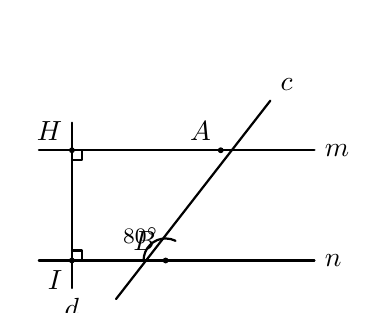
\begin{tikzpicture}[scale=0.7, line cap=round, line join=round]
    % Lines m and n
    \draw[thick] (-2.2, 2.0) -- (2.8, 2.0) node[right] {$m$};
    \draw[thick] (-2.2, 0) -- (2.8, 0) node[right] {$n$};
    % Line d perpendicular at H and I
    \draw[thick] (-1.6, 2.5) -- (-1.6, -0.5) node[below] {$d$};
    \filldraw[black] (-1.6, 2.0) circle (1.2pt) node[above left] {$H$};
    \filldraw[black] (-1.6, 0) circle (1.2pt) node[below left] {$I$};
    \draw[thick] (-1.6, 2.0) ++(0,-0.18) -- ++(0.18,0) -- ++(0,0.18);
    \draw[thick] (-1.6, 0) ++(0,0.18) -- ++(0.18,0) -- ++(0,-0.18);
    % Line c slanted cutting m at A, n at B
    \draw[thick] (2.0, 2.9) node[above right] {$c$} -- (-0.8, -0.7);
    \filldraw[black] (1.1, 2.0) circle (1.2pt) node[above left] {$A$};
    \filldraw[black] (0.1, 0) circle (1.2pt) node[above left] {$B$};
    % Angle ABI = 80
    \draw[thick] (0.1, 0) ++(180:0.4) arc (180:63.4:0.4);
    \node[font=\footnotesize] at (-0.35, 0.45) {$80^\circ$};
\end{tikzpicture}
}
\end{ex}
\vspace{2mm}

\begin{ex}
Một cửa hàng nhập về $100$ xe hơi đồ chơi với giá gốc mỗi cái $300\,000$ đồng. Cửa hàng đã bán $65$ xe với giá mỗi cái lãi $30\%$ so với giá gốc; $35$ cái xe còn lại bán lỗ $7\%$ so với giá gốc. Hỏi sau khi bán hết $100$ xe hơi đồ chơi cửa hàng đó lãi hay lỗ bao nhiêu tiền?
\end{ex}
\vspace{2mm}


\begin{center}
\rule{4cm}{0.4pt}\\
\textit{--- HẾT ---}
\end{center}
\end{document}
